\documentclass[../../../OAE-SPEC-MAIN.tex]{subfiles}
\begin{document}

% STANDALONE


\section{Back to Back Shannon Channels}
\vspace{30px}

\marginnote{From ./AE-Specifications-ETH/Shannon.tex}

\subsection{Two independent Metcalfe Channels (Max flow, no Interaction)}

\begin{figure*}
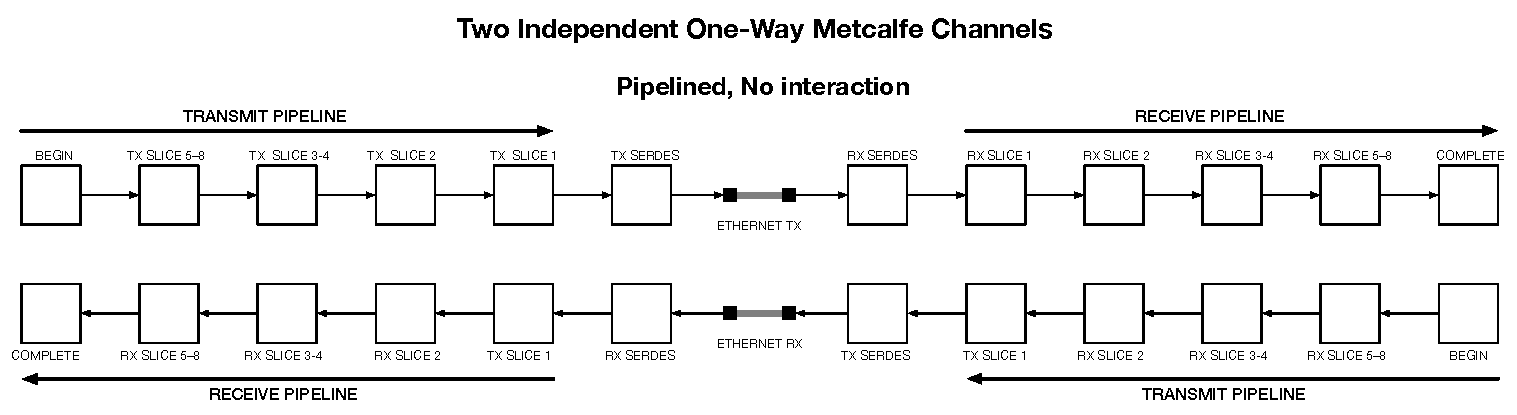
\includegraphics[width=\textwidth]{FIGURES/Two-Independent-Metcalfe.pdf}
  \caption{Two Independent Metcalfe Channels}
\end{figure*}

\vspace{30px}

\subsection{Internal (SACK) Feedback on last slice}

\begin{figure*}
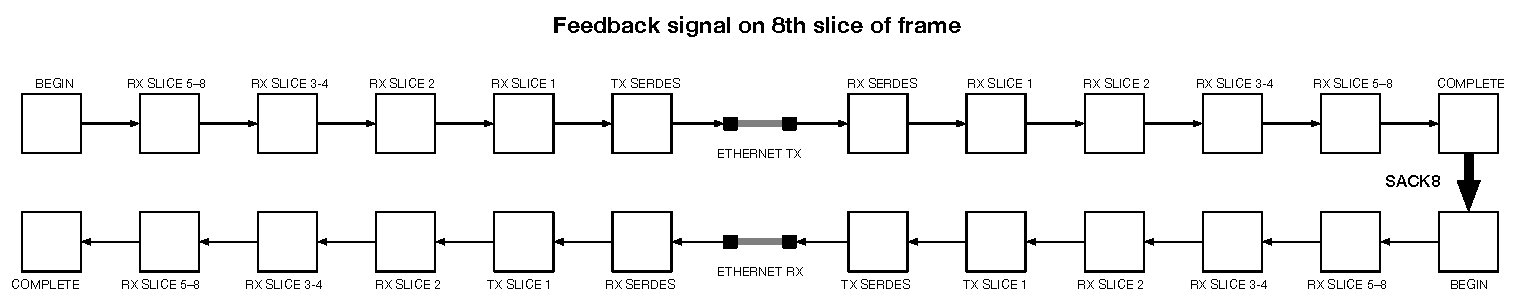
\includegraphics[width=\textwidth]{FIGURES/feedback-slice-8.pdf}
  \caption{Feedback signal on slice 8}
\end{figure*}

\vspace{30px}

\subsection{Internal (SACK) Feedback on first slice}

\marginnote{See SACK description by Sahas \cite{sahas-02025-1}}

\begin{figure*}
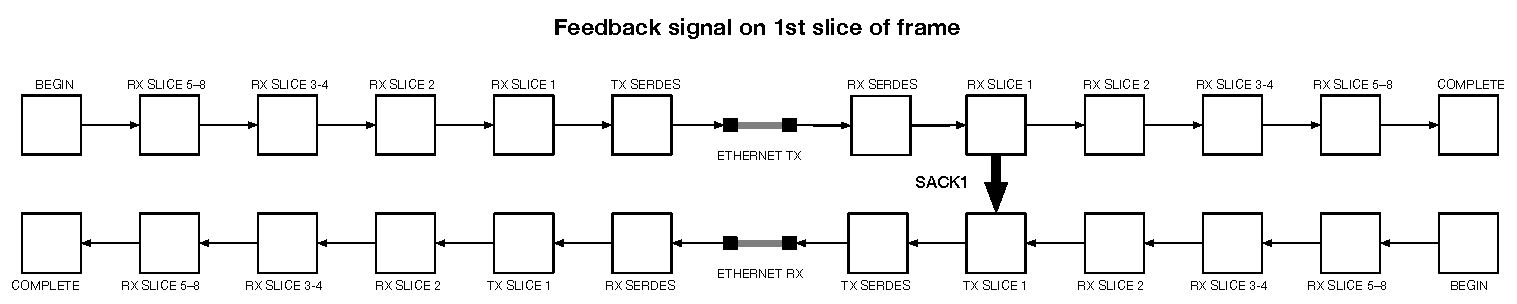
\includegraphics[width=\textwidth]{FIGURES/Feedback-slice-1.pdf}
  \caption{Feedback signal on slice 1}
\end{figure*}

\vspace{30px}

\section{Architectural Framework: Four Shannon-like Levels}

In the proposal for subdividing a 64-byte packet into 8-byte slices, we introduce partial acknowledgments (SACKs) at four (decrementing) boundaries (\texttt{11}, \texttt{10}, \texttt{01}, \texttt{00}). Each of these points reveals an incrementally deeper level of the receiver’s certainty about the data, the hardware, and the appropriate next step in the protocol. We can interpret this progressive certainty in terms of four conceptual \emph{layers} reminiscent of Shannon’s \emph{information} theory, but extended to address knowledge, semantics, and understanding. This layering describes how a receiver (e.g., the SmartNIC) transitions from raw incoming bits to meaningful messages that can be handed off to the host processor.

\marginnote{Back-to-Back (B2B) Shannon Channels are “Perfect Information Feedback” (PIF) as senders see their own transmitted packet returning back from the receiver and thus can detect channel errors.  Thus making CRCs Checksums, Parity and FEC unnecessary.
Similar to "Perfect Information Feedback" in: \href{https://dl.acm.org/doi/pdf/10.1145/1499586.1499751}{Norm Abramson, “Packet switching with satellites,” NCC, 1973}}

\subsection{Layer 1: Information (Surprisal)}

At the first level, information refers to the direct "yes/no" answer to a question of interest: the arrival or non-arrival of bits, which Shannon famously treated as the surprisal of a received symbol. At the SACK \texttt{00} boundary, when the receiver detects the first 8-byte slice without error, it learns that the link is alive and that the data matches expectations (i.e., no immediate mismatch). This is pure information because it distinguishes the event "we did receive slice \#1 correctly" from "we did not." The mutual information gained here confirms a working cable and a functional SerDes.

At this early stage, the question posed is binary: "Did the hardware see valid bits?" The surprisal is that valid bits were received, as opposed to no signal or corrupted data.

\subsection{Layer 2: Knowledge (Captured Information)}

The second layer, knowledge, arises when the raw bits are stored or captured in a meaningful structure. This could be as simple as a recognized slice stored in buffer memory or a pipeline register. By the time the second slice arrives, the receiver has captured more bits—16 bytes in total—and placed them into NIC-internal registers. It can then perform further checks, such as alignment, partial CRC, or checking for expected header fields. The SACK \texttt{01} confirms that the hardware not only saw valid bits but also placed them in the correct buffer location.

At this point, the system has a partial understanding of the data. It knows that the 16 bytes are recognized and safely stored, awaiting deeper logic to interpret them.

\subsection{Layer 3: Semantics (Meaning)}

The third layer, semantics, involves the system deciding what the bits mean in terms of subsequent action. This layer determines which state machine or processing path is relevant for the given data. At the SACK \texttt{10} boundary, after 32 bytes have been received, the NIC has gathered enough information to partially decode the data. For example, it might be able to determine which protocol or message type is indicated. The NIC can confirm that buffer slots or ring descriptors are available and that the correct state machine is loaded (e.g., state machine A for small control frames, or state machine B for streaming payloads).

Once the NIC signals SACK \texttt{10}, the sender learns that the hardware has found the data coherent enough to continue. The semantics are recognized sufficiently to proceed without hazard. The receiver has now moved from simply knowing the bits are correct (Layers 1 and 2) to understanding how to proceed and which internal resources or state machines to activate.

\subsection{Layer 4: Understanding (Syntax)}

The final layer, understanding, refers to the recognition that the message fits into a finite set of concepts or message types that the NIC accepts. This implies that the message has a correct syntax recognized by the hardware. At the SACK \texttt{11} boundary, which occurs when slices 5–8 arrive, the full 64 bytes have been received and match a legitimate frame or message layout. The NIC is now ready to push the message onto the PCIe bus or an internal ring buffer for the host processor.

At this stage, the NIC has a full understanding of the message, knowing exactly how to finalize the packet, classify it, and pass it upstream for higher-level processing. No further layer-2 repairs are needed, and the message is ready for the next step in the protocol.

\section{Bidirectional Shannon Channels}

\begin{figure*}
%  \incplt{acquisition_functions_contours}
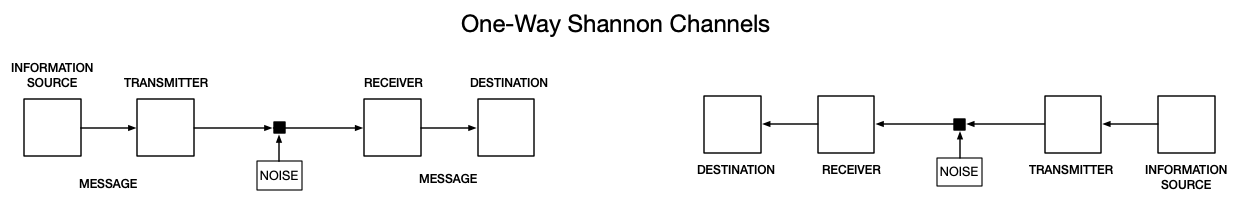
\includegraphics[width=\textwidth]{FIGURES/One-Way-Shannon.png}
  \caption{Shannon One-Way Channels. }
\end{figure*}

Shannon Channels are normally shown in one \emph{direction} of flow -- from Information source to Information Destination. Here we exploit two-way communication (signaling) Back to Back Channels with immediate (slice by slice) feedback. Then the equations tell us something interesting about the \emph{symmetry} of set reconciliation on both sides of the link.

With back-to-back Shannon Channels, with (immediate) slice by slice feedback, we get Perfect Information Transfer (PIT) \cite{soltted-aloha}. We can therefore dispense with Checksums, CRC's, FEC or even Parity,  because the failure modes these EDC and ECC codes address are already covered by PIT.  This has two advantages:

\begin{itemize}
\item The elimination of spatial redundancy on the wire makes the packets shorter
\item The need to calculate increasingly complex codes reduces computation and energy dissipation on the link
\end{itemize}

\marginnote{Redundancy is a poor crutch when  assumptions about uniform probability distributions are violated (which they almost always are in practice).}



\subsection{Metcalfe Half-Duplex}

\begin{figure*}
%  \incplt{acquisition_functions_contours}
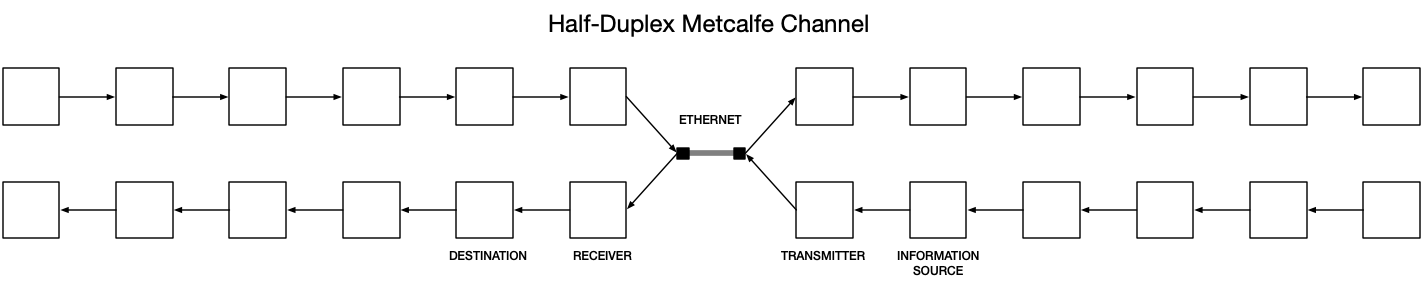
\includegraphics[width=\textwidth]{FIGURES/Half-Duplex-Metcalfe.png}
  \caption{The original Metcalfe + Boggs Ethernet was a bus. A long cable where `stations' were TAPs on the bus. This meant that each station had to both listen, and transmit from teach tap. In this figure we show two \emph{independent} streams of packets going in opposite direction (forwardpropagation and backpropagation) through a single half-duplex link}
\end{figure*}


\vspace{70px}



\vspace{35px}
\begin{figure*}
%  \incplt{acquisition_functions_contours}
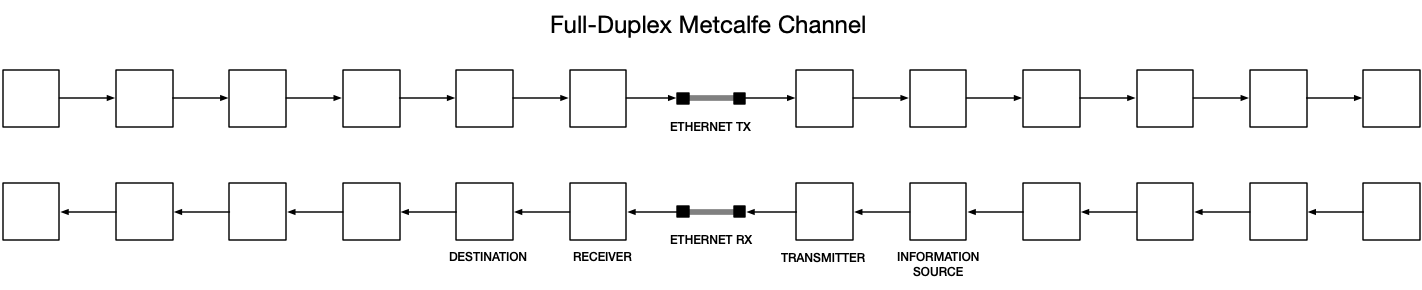
\includegraphics[width=\textwidth]{FIGURES/Full-Duplex-Metcalfe.png}
  \caption{Modern Ethernet Links are bidirectional; two sub-channels: \\one for transmit,  one for receive}
\end{figure*}



\vspace{40px}

\subsection{Full-Duplex Bi-pipelined Shannon-Metcalfe Channel}

\vspace{35px}

\begin{figure*}
%  \incplt{acquisition_functions_contours}

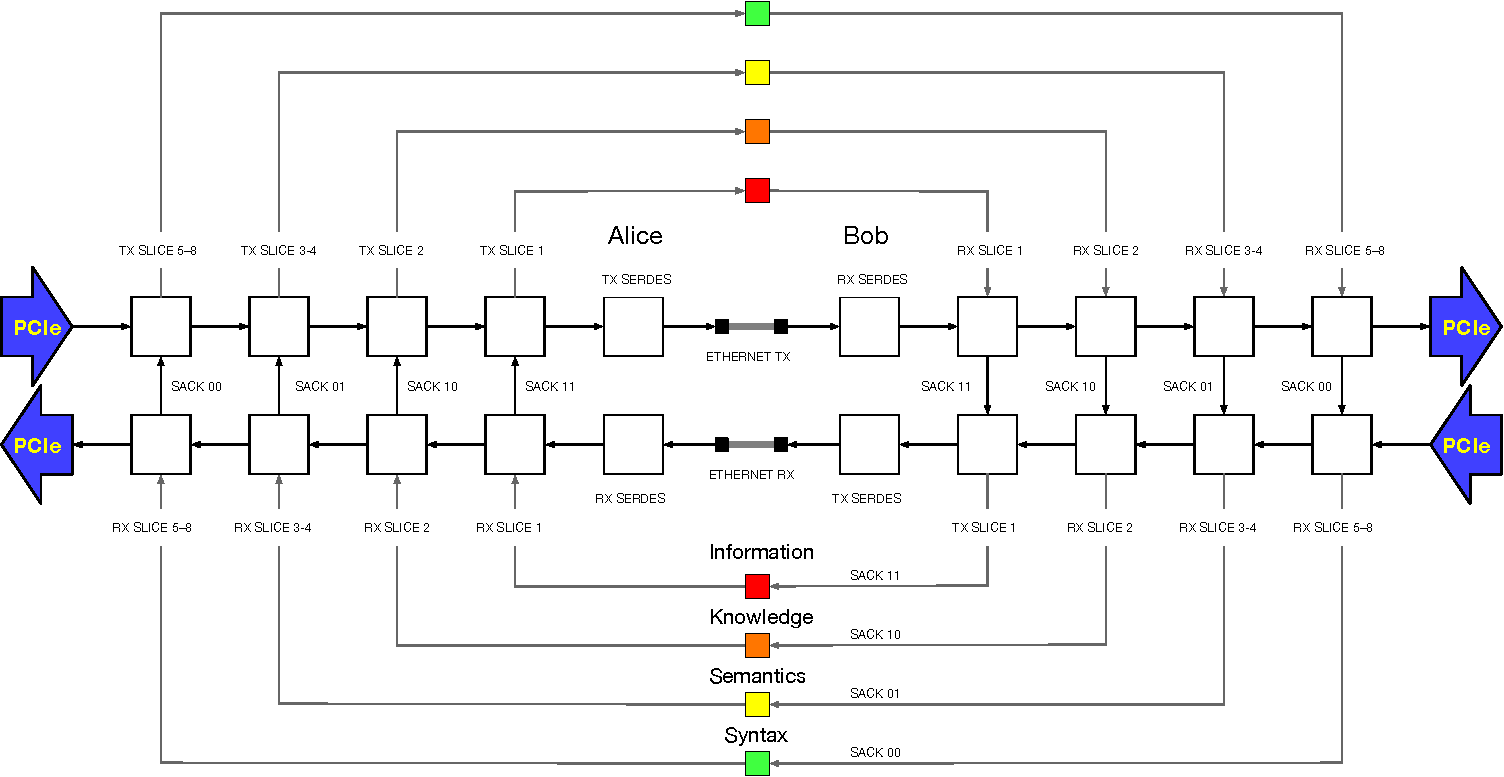
\includegraphics[width=\textwidth]{FIGURES/Full-Duplex-Bi-Pipelined.pdf}
  \caption{Complete model: Bi-pipelined full duplex exchange of  Æthernet frames. Complete with internal "Slice ACKnowledges" (SACKs) -- sequenced with increasing \emph{common knowledge} depth inside SerDes/FPGA}
\end{figure*}

The figure above is a simple, formally verifiable, mathematical description, from API to bits on the wire (Shannon channel). 





\end{document}
